\documentclass[brazilian, 12pt, a4paper, final]{article}
\usepackage[utf8]{inputenc}
\usepackage[brazil]{babel}
\usepackage[T1]{fontenc}
\usepackage{multicol}
\usepackage{graphicx}
\usepackage{indentfirst}
\usepackage{amsmath}
\usepackage{array}
\usepackage{caption}
\usepackage[left=1.5cm, right=1.5cm]{geometry}

\title{\textbf{Trabalho 3: Resolução analítica e numérica para problema de valor inicial}}

\author{Cristiane de Paula Oliveira\\\\\small{Instituto de Física -- Universidade Federal do Rio Grande do Sul}}

\begin{document}

\maketitle

\section{Problema}
Exercicio 29 da seçao 5.4 do livro {\em Análise Numérica} de Richard L. Burden, J. Douglas Faires \& Annette M. Burden, tradução da 10ª edição norte-americana:
\begin{quote}
  Mostre que o método do ponto médio e o método de Euler modificado resultam nas mesmas aproximações para o problema de valor inicial
  \begin{equation*}
    y'=-y+t+1, \;\;\; 0\le t \le 1, \;\;\; y(0)=1,
  \end{equation*}
  \noindent
  para  $h$. Por que isto é verdade?
\end{quote}

\section{Métodos}
Neste trabalho, serão utilizados métodos de Runge-Kutta de segunda ordem. Nesse caso, utiliza-se os três primeiros termos da expansão em séries de Taylor, da forma
\begin{equation}\label{eq:Taylor}
  \omega_{i+1}=\omega_{i} + \frac{d\omega}{dt}\Bigr|_{\substack{(t_i,\omega_i)}}\,h + \frac{1}{2!} \frac{d^2\omega}{dt^2}\Bigr|_{\substack{(t_i,\omega_i)}}\, h^2 + \mathcal{O}(h^3)
\end{equation}

Sendo $\frac{d\omega}{dt}$ uma função conhecida, podemos resolver (\ref{eq:Taylor}) e encontrar uma aproximação numérica.
\begin{equation}\label{eq:RK}
  \omega_{i+1}=\omega_{i}+a_1\,h\,f(t_i,\omega_i) + a_2\,h\,f(t_i+\alpha_2\,h, \omega_i+\delta_2\,h\,f(t_i,\omega_i))
\end{equation}

As constantes $a_1$, $a_2$, $\alpha_2$ e $\delta_2$ devem ser determinadas de forma que:

\[
\begin{cases}
  a_1+a_2=1;\\
  a_2\alpha_2=\frac{1}{2}\\
  a_2\delta_2=\frac{1}{2}
\end{cases}
\]

\subsection{Método do Ponto Médio}
Como existem somente 3 equações para encontrar as 4 incógnitas $a_1$, $a_2$, $\alpha_2$ e $\delta_2$. Portanto, existem várias escolhas dessas constantes para implementar o método de Runge-Kutta de $2^{a}$ ordem. Para o método do ponto médio, os valores das constantes são definidos $a_1=0$, $a_2=1$, $\alpha_2=\delta_2=\frac{1}{2}$.

Assim, a equação (\ref{eq:RK}) fica 
\begin{equation}\label{eq:RKm}
  \omega_{i+1}=\omega_{i}+h\,f\left(t_i+\frac{h}{2}, \omega_i+\frac{h}{2}\, f(t_i,\omega_i)\right)  
\end{equation}
\noindent
onde $f(t,\omega)=\frac{d\omega}{dt}$ e $h=t_{i+1}-t_{i}$.

\subsection{Método de Euler Modificado}
O método de Euler modificado corresponde a outra escolha das constantes, sendo $a_1=a_2=\frac{1}{2}$ e $\alpha_1=\delta_1=1$. Dessa forma
\begin{equation}\label{eq:EM}
  \omega_{i+1}=\omega_{i} + \frac{h}{2}[f(t_i,\omega_i)+f(t_i+h, \omega_i+h\,f(t_i,\omega_i)]
\end{equation}
\noindent
onde $f(t,\omega)=\frac{d\omega}{dt}$ e $h=t_{i+1}-t_{i}$.

\section{Resolução analítica}
Para a resolução analítica, utiliza-se a notação  correspondente ao problema $y=\omega$ e $y'=f(t,\omega)$.

Sendo $f(t,y)=-y+t+1$, encontra-se $y_{i+1}$ pelo método do Ponto Médio conforme a equação (\ref{eq:RKm}).

\begin{eqnarray}
  y_{i+1}&=&y_i+h\, f(t_i+\frac{h}{2},y_i+\frac{h}{2}\,f(t_i,y_i)) \nonumber \\
  &=&y_i+h\, f(t_i+\frac{h}{2}, y_i+\frac{h}{2}(-y_i+t_i+1)) \nonumber \\
  &=&y_i+h\, [-(y_i-\frac{h}{2}y_i+\frac{h}{2}t_i+\frac{h}{2})+t_i+\frac{h}{2}+1] \nonumber \\
  &=&y_i+h\,(-y_i+\frac{h}{2}y_i-\frac{h}{2}t_i-\frac{h}{2}+ti+\frac{h}{2}+1) \nonumber \\
  &=&y_i-hy_i+\frac{h^2}{2}y_i-\frac{h^2}{2}t_i+ht_i+h \nonumber \\
  y_{i+1}&=&y_i+\left(\frac{h^2}{2}-h\right)y_i+\left(h-\frac{h^2}{2}\right)t_i+h \label{eq:5}
\end{eqnarray}

Utilizando-se o método de Euler Modificado, conforme a equação (\ref{eq:EM}), obtém-se

\begin{eqnarray}
  y_{i+1}&=&y_i+\frac{h}{2}\, f(t_i,y_i)+\frac{h}{2}\, f(t_i+h,y_i+h\,f(t_i,y_i)) \nonumber \\
  &=&y_i+\frac{h}{2}(-y_i+t_i+1)+\frac{h}{2}\,f(t_i+h,y_i+h(-y_i+t_i+1)) \nonumber \\
  &=&y_i-\frac{h}{2}y_i+\frac{h}{2}t_i+\frac{h}{2}+\frac{h}{2}\,f(t_i+h,y_i-hy_i+ht_i+h) \nonumber \\
  &=&y_i-\frac{h}{2}y_i+\frac{h}{2}t_i+\frac{h}{2}+\frac{h}{2}\,[-(y_i-hy_i+ht_i+h)+t_i+h+1] \nonumber \\
  &=&y_i-\frac{h}{2}y_i+\frac{h}{2}t_i+\frac{h}{2}+\frac{h}{2}\,(-y_i+hy_i-ht_i-h+t_i+h+1) \nonumber \\
  &=&y_i-\frac{h}{2}y_i+\frac{h}{2}t_i+\frac{h}{2}-\frac{h}{2}y_i+\frac{h^2}{2}y_i-\frac{h^2}{2}t_i+\frac{h}{2}t_i+\frac{h}{2} \nonumber \\
  &=&y_i-hy_i+ht_i+h+\frac{h^2}{2}y_i-\frac{h^2}{2}ti \nonumber \\
  y_{i+1}&=&y_i+\left(\frac{h^2}{2}-h\right)y_i+\left(h-\frac{h^2}{2}\right)t_i+h \label{eq:6}
\end{eqnarray}

Nota-se que a equação (\ref{eq:5}) é idêntica à equação (\ref{eq:6}). Isso ocorre pois os dois métodos são de Runge-Kutta de ordem 2. Para este problema em específico, os dois métodos resultam na mesma aproximação para qualquer escolha de $h$.

Para ser possível estimar os erros envolvidos nos métodos, resolvemos o problema de valor inicial para encontrar $y(t)$. A solução exata para este problema é
\begin{equation}
  y(t)=\mathrm{e}^{-t}+t
\end{equation}

\section{Verificação numérica}
Utilizando um programa que resolve a equação diferencial do problema pelo método do ponto médio e pelo método de Euler modificado, encontra-se uma solução numérica. Essas soluções numéricas são mostradas na na figura \ref{fig:solmid}, para o método do ponto médio, e na figura \ref{fig:soleul}, para o método de Euler modificado.

Optou-se por usar $h=0,1$ nestes gráficos porque, como pode-se perceber pela figura \ref{fig:erro}, os erros com esse valor de $h$ são toleráveis.

\begin{figure}[htbp]
  \centering
  \includegraphics[width=0.50\textwidth,angle=-90]{solucao_mid.eps}
  \caption{Comparação entre a solução numérica do problema e a solução exata (equação (7)) utilizando o método do ponto médio.}
  \label{fig:solmid}
\end{figure}

\begin{figure}[htbp]
  \centering
  \includegraphics[width=0.50\textwidth,angle=-90]{solucao_eul.eps}
  \caption{Comparação entre a solução numérica do problema e a solução exata (equação (7)) utilizando o método de Euler modificado.}
  \label{fig:soleul}
\end{figure}


Na figura \ref{fig:mideul} mostra-se a subtração entre as soluções encontrada por cada método ao longo do intervalo $0\le t \le 1$. Pela resolução analítica do problema, espera-se que os valores encontrados em ambos os métodos sejam idênticos.

Porém, percebe-se que isso não acontece numericamente. Isso ocorre pois na realidade existe um erro numérico de representação do ponto flutuante. Como as operações realizadas por cada método são diferentes, a conversão de um número real para dígitos binários pode gerar um erro que é acumulado. No gráfico, até o ponto $t=0,5$ os resultados são  de fato idênticos, aumentando a diferença entre eles a partir desse ponto. Para outros problemas, essa diferença, da ordem de $10^{-16}$, pode ser bastante significativa.

\begin{figure}[htbp]
  \centering
  \includegraphics[width=0.50\textwidth,angle=-90]{mid_eul.eps}
  \caption{Diferença entre a solução numérica encontrada pelo método do ponto médio e pelo método de Euler modificado.}
  \label{fig:mideul}
\end{figure}

\section{Análises dos erros}
O método de Runge-Kutta de 2ª ordem tem erro local de truncamento $\mathcal{O}(h^3)$ e erro global $\mathcal{O}(h^2)$.

\begin{figure}[htbp]
  \centering
  \includegraphics[width=0.50\textwidth,angle=-90]{erros.eps}
  \caption{Erro para cada $t$ no intervalo para os métodos do ponto médio e Euler modificado.}
  \label{fig:erro}
\end{figure}

Nas figuras \ref{fig:hmid} e \ref{fig:heul} são mostrados o erro global para difentes valores de $h$. Os valores no eixo vertical estão em logaritmo base 10 do valor absoluto do erro e no eixo horizontal em logaritmo base 10 de $h$.

Ajusta-se uma reta da forma $f(x)=C+n\,x$, onde $f(x)=\log _{10}erro$, $x=\log_{10}h$, $C$ o ponto onde $\log_{10}h=0$, e $n$ é a potência de $h$, isto é, a ordem do erro global.

A partir dos resultados, encontrau-se que quando $\log_{10}h=0$, e portanto $h=1$, $\log_{10}erro\approx-0,87903$. Portanto, ajustou-se a reta $f(x)=-0,87903 + n\,x$  para encontrar somente o valor de $n$.

Para o ajuste da figura \ref{fig:hmid}, onde mostra-se o erro global obtido pelo método do ponto médio, encontrou-se que $n=2,09017\pm0,0176$.

\begin{figure}[htbp]
  \centering
  \includegraphics[width=0.50\textwidth,angle=-90]{h_erros_mid.eps}
  \caption{Erro global para diferentes valores de $h$. A inclinação da reta é $n=2,09017\pm0,0176$.}
  \label{fig:hmid}
\end{figure}

O erro global encontrado pelo método de Euler modificado é mostrado na figura \ref{fig:heul}. Novamente, ajustou-se uma reta cuja inclinação foi de $n=2,09004\pm0,01763$.

\begin{figure}[htbp]
  \centering
  \includegraphics[width=0.50\textwidth,angle=-90]{h_erros_eul.eps}
  \caption{Erro global para diferentes valores de $h$. A inclinação da reta é $n=2,09004\pm0,01763$.}
  \label{fig:heul}
\end{figure}

Espera-se $n=2$ para métodos de Runge-Kutta 2ª ordem. Os resultados de ambos ajustes concordam com a expectativa teórica. Esses valores não são idênticos porque, como já foi discutido anteriormente, há um acúmulo de erro na representação de ponto flutuante.

\begin{thebibliography}{n}
\bibitem{Burden_book} RICHARD L. BURDEN, J. DOUGLAS FAIRES e ANNETTE M. BURDEN. {\em Análise Numérica}, (editora Cengage Learning,  tradução da 10ª edição norte-americana, 2016)
  
\end{thebibliography}

\appendix
\section{APÊNDICE - INSTRUÇÕES}

Para compilar e rodar todos os programas utiliza-se o script:
\begin{verbatim}
$ sh RunT3.sh
\end{verbatim}

Ao final, plota-se os gráficos utilizando:
\begin{verbatim}
gnuplot> load 'PlotAll.gnu'
\end{verbatim}

\end{document}
